% XeLaTeX can use any Mac OS X font. See the setromanfont command below.
% Input to XeLaTeX is full Unicode, so Unicode characters can be typed directly into the source.

% The next lines tell TeXShop to typeset with xelatex, and to open and save the source with Unicode encoding.

%!TEX TS-program = xelatex(
%!TEX encoding = UTF-8 Unicode

\documentclass{article}
\usepackage{xr-hyper}
\usepackage{hyperref}
\usepackage[margin=15mm,landscape,a4paper]{geometry}                % See geometry.pdf to learn the layout options. There are lots.
%\geometry{a5paper}                   % ... or a4paper or a5paper or ... 
%\geometry{landscape}                % Activate for for rotated page geometry
\usepackage[parfill]{parskip}    % Activate to begin paragraphs with an empty line rather than an indent
\usepackage{graphicx}
\usepackage[french]{babel}
\usepackage{amssymb}
\usepackage{color}
\usepackage{multicol}
\usepackage{cclicenses}
\usepackage{fontspec,xltxtra,xunicode}
\defaultfontfeatures{Mapping=tex-text}
\setromanfont[Mapping=tex-text]{Hoefler Text}
\setsansfont[Scale=MatchLowercase,Mapping=tex-text]{Gill Sans}
\setmonofont[Scale=MatchLowercase]{Andale Mono}

\title{\textbf{Aide-mémoire Scilab}}
\author{Christophe Saint-Jean}
\date{version du \today}

\begin{document}
\begin{multicols}{3}
\maketitle

\textit{Cette aide-mémoire Scilab est mis à disposition selon les termes de la licence Creative Commons Attribution - Pas d’Utilisation Commerciale 3.0 France. \ccby\ccnc\cc}
\section{Généralités}
\subsection{Conventions de cette aide-mémoire}
\begin{description}
\item{c*} sont des variables ou des expressions scalaires.
\item{v*} sont des variables ou des expressions vectorielles.
\item{M*, N et P} représentent des valeurs ou des expressions matricielles.
\item{str*} sont des valeurs ou des expressions de type chaînes de caractères.
\item{cond*} sont des valeurs ou des expressions booléennes.
\item{cmd*} sont des valeurs ou des expressions booléennes.
\item{var*} sont des variables ou des expressions sans type spécifique.
\end{description}
\subsection{Aide}
\begin{description}
\item{\textbf{help}()} démarre le système d'aide
\item{\textbf{help} (\textit{str\_cmd})} recherche l'aide sur la fonction \textit{cmd}
       \begin{verbatim}--> help ('inv')\end{verbatim}
\item{\textbf{apropos}(\textit{str\_kwd})} recherche dans l'aide le mot-clé \textit{kwd} et ordonne par pertinence les résultats
       \begin{verbatim}--> apropos('inv')\end{verbatim}
\end{description}
\subsection{Environnement}
\label{environnement}
\begin{description}
\item{\textbf{who}} liste les variables connues dans l'environnement.
\item{\textbf{whos}} liste de manière détaillée les variables connues dans l'environnement.      
\item{\textbf{clear}(\textit{str\_var1}, \textit{str\_var2}, \ldots, \textit{str\_varn})} supprime les variables \textit{var1},\textit{var2}, \ldots, \textit{varn} de l'environnement.
\begin{verbatim}--> clear('M','n','i')\end{verbatim}
\item{\textbf{clear}()} supprime toutes les variables.
\item{\textbf{load}(\textit{str\_fichier})} charge les variables sauvegardées dans \textit{fichier}.
\item{\textbf{save}(\textit{str\_fichier})} sauvegarde l'ensemble des variables dans \textit{fichier}.
\item{\textit{c\_id} = \textbf{diary}(\textit{str\_fichier})} ouvre le journal \textit{id} dans le fichier et sauvegarde les commandes entrées dans la console.
\item{\textbf{diary}(\textit{c\_id},'close')} sauve le journal \textit{id}.
\begin{verbatim}
-->id = diary('TP1.txt')
 id  =
    1.  
--> // des commandes
-->diary(id,'close')
\end{verbatim}
\item{\textbf{ls}()} liste des fichiers du répertoire de travail.
\item{\textbf{pwd}()} affiche le répertoire courant.
\item{\textbf{cd}(\textit{str\_rep})} modifie le répertoire courant (-> \textit{rep}).
\item{\textbf{exec} (\textit{str\_script})} exécute le fichier de commandes \textit{script}.
\begin{verbatim}
-->exec('TP1.sce')
\end{verbatim}
\item{\textbf{scinotes}()} lance l'éditeur de texte intégré de Scilab.
\end{description}
\subsection{Constantes}
\label{constantes}
\begin{description}
\item{\textbf{\%i}, \textbf{\%pi}, \textbf{\%e}}:  imaginaire $i$, $\pi$, $e$
\item{\textbf{\%eps}} est un petit nombre réel représentable en machine.
\item {\textbf{\%t}, \textbf{\%f}} sont les deux valeurs booléennes \textit{vrai}, \textit{faux}
\item {\textbf{\%inf}} représente $+\infty$ 
\item {\textbf{\%nan}}  indique qu'une valeur n'est pas déterminée.
\begin{verbatim}
-->%inf/%inf
 ans  =
    Nan
\end{verbatim}
\item {\textbf{isnan}(\textit{M}), \textbf{isinf}(\textit{M})} teste chaque élément de \textit{M}.
\begin{verbatim} 
-->M = [%nan 1; -2 %nan]; isnan(M)
 ans  =
  T F  
  F T 
  \end{verbatim}
\end{description}
\subsection{Autres fonctions}
\label{autres}
\begin{description}
\item\label{disp}{\textbf{disp}(\textit{var1}, \textit{var2}, \ldots, \textit{varn})} affiche chacun des paramètres dans l'ordre \textit{varn}, \ldots, \textit{var2},\textit{var1}.
\begin{verbatim}
-->a=3;b=5;disp('Un petit texte :',a,a+b)
    8.  
    3.  
 Un petit texte : 
\end{verbatim}
\item\label{input}{\textit{c} = \textbf{input}(\textit{str\_msg})} permet de récupérer une valeur saisie par l'utilisateur.
\begin{verbatim}
-->h=input('Donnez une valeur pour h : ');
Donnez une valeur pour h : 6
-->disp(h)
    6
\end{verbatim}
\end{description}

\section{Vecteurs et matrices}
\subsection{Définition}
\label{vecteurs}
\begin{description}
\item{\textbf{[ ]}} est la matrice vide.
\item{\textbf{[}\textit{c1, c2,~\ldots ,~cn}\textbf{]} ou \textbf{[}\textit{c1 c2 \ldots ~cn}\textbf{]}} est un vecteur ligne.
\begin{verbatim}
-->[1 2 3]  
 ans  =
    1.    2.    3. 
\end{verbatim}
\item{\textbf{[}\textit{c1; c2;~\ldots ;~cn}\textbf{]}} est un vecteur colonne.
\begin{verbatim}
-->[1 ; 2 ; 3]  
 ans  =
    1.
    2.
    3. 
\end{verbatim}
\item{\textbf{[}\textit{v1, v2,~\ldots ,~vn}\textbf{]} ou \textbf{[}\textit{v1 v2 \ldots ~vn}\textbf{]}} est une matrice à n colonnes si les vecteurs colonnes \textit{v1, v2,~\ldots ,~vn} sont de même longueur.
\begin{verbatim}
-->[ [1;2;3] [4;5;6] ]
 ans  = 
    1.    4.  
    2.    5.  
    3.    6.
\end{verbatim}   
\item{\textbf{[}\textit{v1; v2;~\ldots ;~vn}\textbf{]}} est une matrice à n lignes si les vecteurs ligne \textit{v1, v2,~\ldots ,~vn} sont de même longueur.
\begin{verbatim}
-->[[1 2 3];[4 5 6]]  
 ans  =
    1.    2.    3.  
    4.    5.    6.  
\end{verbatim}
\item{\textbf{[}\textit{M1; M2;~\ldots ;~Mn}\textbf{]}} est une matrice $(l_{1}+l_{2}+\ldots+l_{n}) \times c$ si les matrices \textit{M1, M2,~\ldots ,~Mn} sont de taille $l_{i} \times c$.
\begin{verbatim}
-->M1 = [[1 2] ; [3 4]], M2 = [5 6], [M1 ; M2]
 M1  =
    1.    2.  
    3.    4.  
 M2  = 
    5.    6.  
 ans  =
    1.    2.  
    3.    4.  
    5.    6  
\end{verbatim}
\item{\textbf{[}\textit{M1~M2~\ldots ~Mn}\textbf{]}} est une matrice $l \times (c_{1}+c_{2}+\ldots+c_{n})$ si les matrices M1, M2,~\ldots ,~Mn sont de taille $l \times c_{i}$.
\begin{verbatim}
-->M1 = [[1 2] ; [3 4]], M2 = [5;6], [M1 M2]
 M1  =
    1.    2.  
    3.    4.  
 M2  =
    5.  
    6.  
 ans  =
    1.    2.    5.  
    3.    4.    6.  
\end{verbatim}
\end{description}
\subsection{Cas particuliers}
\begin{description}
\item{\textbf{ones}(\textit{c\_lig},1)} est le vecteur \textit{lig} $\times$ 1 rempli de 1.
\item{\textbf{ones}(1,\textit{c\_col})} est le vecteur \textit{1} $\times$  \textit{col} rempli de 1.
\item{\textbf{ones}(\textit{c\_lig},\textit{c\_col})} est la matrice $lig \times col$ remplie de 1.
\item{\textbf{zeros}(\textit{c},1),\textbf{zeros}(1,\textit{c}), \textbf{zeros}(\textit{c\_lig},\textit{c\_col})}  idem avec des 0.
\item{\textbf{eye}(\textit{c},\textit{c})} est la matrice identité $I_{c}$.
\item{\textit{c\_deb}\textbf{:} \textit{c\_fin}} produit la séquence des nombres vérifiant
$$ [deb,fin] \cap [deb,deb+1,deb+2,\ldots]$$
\begin{verbatim}
-->1:4
 ans  =
    1.    2.    3.    4.  
-->1:-2
 ans  =
     []
-->2.5:5
 ans  =
    2.5    3.5    4.5 
\end{verbatim}
\item{\textit{c\_deb}\textbf{:} \textit{c\_pas}\textbf{:} \textit{c\_fin}} produit la séquence des nombres vérifiant
$$ [deb,fin] \cap [deb,deb+pas,deb+2*pas,\ldots]$$
\begin{verbatim}
-->1:1:4
 ans  =
    1.    2.    3.    4.  
-->4:-1:1
 ans  =
    4.    3.    2.    1.  
-->0:%pi/4:%pi
 ans  =
    0.    0.785    1.571    2.356    3.142
\end{verbatim}
\item{\textbf{linspace}(\textit{c\_deb},\textit{c\_fin},\textit{c\_n})} produit \textit{n} nombres linéairement répartis dans l'intervalle $[deb,fin]$.
\item{\textbf{logspace}(\textit{c\_deb},\textit{c\_fin},\textit{c\_n})}  produit \textit{n} nombres logarithmiquement répartis dans l'intervalle $[deb,fin]$.
\begin{verbatim}
-->linspace(2,4,3)
 ans  =
    2.    3.    4.  
-->logspace(2,4,3)
 ans  =
    100.    1000.   10000.
-->10^linspace(2,4,3)
 ans  =
    100.    1000.   10000. 
\end{verbatim}
\item{\textbf{diag}($M$)} est le vecteur des éléments diagonaux de $M$.
\item{\textbf{diag}($v$)} est une matrice carrée diagonale à partir de $v$.
\item{\textbf{rand}(\textit{c\_lig},\textit{c\_col})} retourne une matrice de taille $lig \times col$ dont les entrées sont choisis aléatoirement (uniformément dans $[0,1]$).
\begin{verbatim}
-->rand(2,3)
 ans  =
    0.728    0.547    0.740  
    0.268    0.989    0.004 
\end{verbatim}
\item{\textbf{rand}(\textit{M})} retourne une matrice de même taille que $M$ dont les entrées sont choisis aléatoirement (uniformément dans $[0,1]$).

\end{description}
\subsection{Propriétés}
\begin{description}
\item{\textbf{length}($v$)} retourne le nombre d'éléments de $v$.
\item{\textbf{length}($M$)} retourne le nombre d'éléments de la matrice $M$.
\item{\textbf{size}($M$)} est le vecteur du nombre d'éléments par dimension de la matrice $M$.
\item{[\textit{c\_lig},\textit{c\_col} ] = \textbf{size}($M$)} permet d'extraire directement le nombre de lignes $lig$ et de colonnes $col$ de la matrice $M$.
\begin{verbatim}
-->M =rand(3,2); length(M)
 ans  =
    6.  
-->size(M)
 ans  =
    3.    2.  
-->[l,c]=size(M)
 c  =
    2.  
 l  =
    3.
\end{verbatim}
\end{description}
\subsection{Indexation}
\begin{description}
\item{$v$\textbf{(}1\textbf{)}, $v$\textbf{(}\textit{c\_i}\textbf{)}, $v$\textbf{(\$)}} désignent le premier, le $i^{ieme}$ et le dernier élément du vecteur $v$.
\item{$v$\textbf{(}1\textbf{:}\textit{c\_i}\textbf{)}} est le vecteur des i premiers éléments du vecteur $v$.
\item{$v$\textbf{(\$-}\textit{c\_i}\textbf{:\$)}} est le vecteur des i+1 derniers éléments du vecteur $v$.
\item{$v$\textbf{(}\textit{v\_ind}\textbf{)}} est un vecteur d'éléments extraits de $v$ à partir du vecteur $ind$ de leurs indices.
\begin{verbatim}
-->v=[2 4 -1 4 1];
-->[v(1) v(3) v($)]
 ans  =
    2.  - 1.  1.
    -->v(1:3)
 ans  =
    2.  4.  - 1. 
-->v($-2:$)
 ans  =
  - 1.  4.  1.
-->v([1 4 3 2 2])
 ans  =
    2.  4. - 1.  4.  4. 
\end{verbatim}
\item{$v$\textbf{(}\textit{v\_TF}\textbf{)}} est un vecteur d'éléments extraits de $v$ à partir du vecteur booléen \textit{TF}.
\begin{verbatim}
-->v=[2 4 -1 4 1];
-->v > 1
 ans  =
  T T F T F  
-->v(v>1)
 ans  =
    2.  4.  4.
\end{verbatim}
\item{$M$\textbf{(}$i$,$j$\textbf{)}} désigne l'élément de $M$ à ligne $i$, colonne $j$.
\item{$M$\textbf{(}$i$,\textbf{:)}} désigne la $i^{ieme}$ ligne de la matrice $M$.
\item{$M$\textbf{(:},$j$\textbf{)}} désigne la $j^{ieme}$ colonne de la matrice $M$.
\begin{verbatim}
-->M = [1 0 4;-2 1 2]
 M  =
    1.  0.  4.  
  - 2.  1.  2.  
-->M(1,:)
 ans  =
    1.  0.  4.  
-->M(:,2)
 ans  = 
    0.  
    1.
\end{verbatim}
\item{$M$\textbf{(:)}} est le vecteur colonne des éléments de $M$ (indice linéaire).
\item{M\textbf{(}\textit{c\_i}\textbf{)}} est le $i^{ieme}$ élément en indice linéaire de $M$.
\begin{verbatim}
-->M = [1 0;-2 1]; M(:)
 ans  =
    1.  
  - 2.  
    0.  
    1.  
-->M(3)
 ans  =
    0.
\end{verbatim}
\item{$M$\textbf{(}\textit{v\_I},\textit{v\_J}\textbf{)}} est une sous-matrice de $M$ à partir des vecteurs $I$ et $J$ de leurs indices ligne et colonne.
\begin{verbatim}
-->M = round(12*rand(3,3)-3)
 M  =
    0.  0. -1.  
  - 1. -2.  5.  
    6.  5.  7.
-->M(1:2,1:2)
 M  =
    0.  0.  
  - 1. -2.
-->M([1,3],[2 3 2])
 ans  = 
    0. -1. 0.  
    5.  7. 5. 
\end{verbatim}
\end{description}

\subsection{Transformations}
\begin{description}
\item{\textbf{flipdim}($v$,1)} inverse l'ordre des éléments du vecteur $v$.
\item{\textbf{flipdim}($M$,\textit{c\_dim})} retourne la matrice $M$ selon la dimension \textit{dim}.
\item{\textbf{matrix}($v$,\textit{c\_lig},\textit{c\_col})} retourne une matrice de taille $lig \times col$ à partir des valeurs de $v$.
\item{\textbf{matrix}($M$,\textit{c\_lig},\textit{c\_col}) ou \textbf{matrix}(M,[\textit{c\_lig},\textit{c\_col}])} retourne une matrice $lig \times col$ à partir des valeurs de $M$.
\begin{verbatim}
-->v=1:6;M = matrix(v,2,3)
 ans  =
    1.  3   5.  
    2.  4.  6. 
-->matrix(M,3,2)
 ans  =
    1.  4.  
    2.  5.  
    3.  6.
\end{verbatim}
\item{\textbf{repmat}($M$,\textit{c\_lig}, \textit{c\_col}) ou \textbf{repmat}($M$,[\textit{c\_lig}, \textit{c\_col}])}\\ retourne une matrice $(lig * n) \times (col * m)$  par recopie de la matrice $M$ de taille $n \times m$.
\begin{verbatim}
-->M = [1 2 ; 3 4]
 M  =
    1.  2.  
    3.  4.  
-->repmat(M,2,3)
 ans  =
    1.  2.  1.  2.  1.  2.  
    3.  4.  3.  4.  3.  4.  
    1   2.  1.  2.  1.  2.  
    3.  4.  3.  4.  3.  4.
\end{verbatim}
\end{description}
\subsection{Autres fonctions utiles}
\begin{description}
\item{\textbf{find}($v$)} retourne les indices de valeurs de $v$ différentes de 0.
\item{\textbf{find}($M$)} retourne les indices linéaires de valeurs de $M$ 
différentes de 0.
\item{[\textit{v\_I},\textit{v\_J}] = \textbf{find}($M$)} retourne les indices ligne $I$ et colonne $J$  des valeurs de $M$ différentes de 0.
\begin{verbatim}
-->v = [2, 0, 1, 0 , -1, 3]
 v  =
    2.  0.  1.  0.  - 1.  3
-->find(v)
 ans  =
    1.  3.  5.  6.
-->find(matrix(v,2,3))
 ans  =
    1.  3.  5.  6.
-->[I,J] = find(matrix(v,2,3))
 J  =
    1.  2.  3.  3.  
 I  =
    1.  1.  1.  2. 
\end{verbatim}
\item{\textbf{find}(\textit{v\_b}), \textbf{find}(\textit{M\_b}),  [\textit{v\_I},\textit{v\_J}] = \textbf{find}(\textit{M\_b})} idem pour les vecteurs et matrices booléennes aves les valeurs \%t.
\item{\textbf{and}(\textit{v\_b})} retourne \%t ssi tous les éléments de $b$ sont \%t (quantificateur universel $\forall$).
\item{\textbf{and}(\textit{v\_b})} retourne \%t ssi tous les éléments de $b$ sont différents de 0.
\item{\textbf{or}(\textit{v\_b})} retourne \%t ssi au moins un élément de $b$ est \%t (quantificateur existentiel $\exists$).
\item{\textbf{or}(\textit{v\_b})} retourne \%t ssi au moins un élément de $b$ est différent de 0.
\begin{verbatim}
-->v = [2, 0, 1, 0 , -1, 3]
 v  =
    2.  0.  1.  0. - 1.  3.  
-->v>0
 ans  =
  T F T F F T  
-->[and(v>0) or(v<0)]
 ans  =
  F T
\end{verbatim}
\end{description}
\section{Math}
\subsection{Calculs élémentaires}
\begin{description}
\item{\textbf{sin,cos,tan,asin,acos,atan,atan2,log,log10,exp,sqrt}}\\
diverses fonctions mathématiques
\begin{verbatim}
-->format(6); v = linspace(0,0.5,6)*%pi
 v  =
    0.  0.314  0.628  0.942  1.257  1.571  
-->sin(v)
 ans  =
    0.  0.309  0.588  0.809  0.951  1.
\end{verbatim}
\item{\textbf{min}($v$)} retourne le minimum d'un vecteur \textit{v}.
\item{[\textit{c\_min},\textit{c\_i}] = \textbf{min}($v$)} idem avec $i$ l'indice du minimum (le $1^{er}$)
\begin{verbatim}
-->v = [2 3 1 2 1]; [m,i] = min(v)
 i  =
    3.  
 m  =
    1. 
\end{verbatim}
\item{\textbf{min}($M$)} retourne le minimum d'une matrice \textit{M}.
\item{\textbf{min}($M$,'c')} retourne le vecteur (colonne) des minima par ligne d'une matrice \textit{M}.
\item{[\textit{v\_min},\textit{v\_I}]=\textbf{min}($M$,'c')} idem avec $I$(j) l'indice du minimum pour la ligne $j$.
\item{\textbf{min}($M$,'r')} retourne le vecteur (ligne) des minima par colonne d'une matrice \textit{M}.
\item{[\textit{v\_min},\textit{v\_I}]=\textbf{min}($M$,'r')} idem avec $I$(j) l'indice du minimum pour la colonne j.
\item{\textbf{max}($v$), \ldots, \textbf{max}($M$,'r')} idem pour le maximum.
\item{\textbf{sum}($v$)} donne la somme du vecteur $v$.
\item{\textbf{sum}($M$)} donne la somme des éléments de la matrice M.
\item{\textbf{sum}($M$,'r') ou \textbf{sum}($M$,1)} retourne le vecteur ligne des sommes par colonne.
\item{\textbf{sum}($M$,'c') ou \textbf{sum}($M$,2)} retourne le vecteur colonne des sommes par ligne.
\item{\textbf{prod}($v$),\ldots, \textbf{prod}($M$,'c')} idem pour le produit.
\item{\textbf{cumsum}($v$)} retourne le vecteur $w$ tel que $$w(j) = \sum_{i=1}^{j} v(i)$$ 
\begin{verbatim}
-->v = 1:5; w = cumsum(v)
 w  =
    1.  3.  6.  10.  15.  
\end{verbatim}
\item{\textbf{cumprod}($v$)} retourne le vecteur $w$ tel que $$w(j) = \prod_{i=1}^{j} v(i)$$
\begin{verbatim}
-->v = 1:5; w = cumprod(v)
 w  =
   1.  2.  6.  24.  120.   
\end{verbatim}
\item{\textbf{diff}($v$)} retourne le vecteur des différences successives de v.
$$w(j) = v(j+1)-v(j)$$
\begin{verbatim}
-->v = 1:5; w = diff(v)
 w  =
    1.  1.  1.  1.  
\end{verbatim}
\item{\textbf{mean}($v$) ou \textbf{mean}($M$)}  retourne la moyenne des éléments d'un vecteur ou d'une matrice.
\item{\textbf{median}($v$) ou \textbf{median}($M$)}  est l'élément médian d'un vecteur ou d'une matrice.
\item{\textbf{unique}($v$)} extrait les éléments de $v$ sans doublons (pas en place).
\item{\textbf{union}(\textit{v\_A},\textit{v\_B}), \textbf{intersect}(\textit{v\_A},\textit{v\_B})}
\item{\textbf{setdiff}(\textit{v\_A},\textit{v\_B}), \textbf{setequal}(\textit{v\_A},\textit{v\_B})} sont les opérations ensemblistes.
\item{\textbf{gsort}($v$)} trie les éléments de $v$ par ordre décroissant.
\item{\textbf{gsort}($v$,'g','i')}  trie les éléments de $v$ par ordre croissant.
\end{description}
\section{Calcul matriciel}
\begin{description}
\item{$M$\textbf{'}} est la matrice adjointe de $M$.
\item{$M$\textbf{.'}} est la transposée de $M$.
\item{$M$\textbf{ + }$N$ et $M$\textbf{ - }$N$} sont la somme et la soustraction de $M$ et $N$.
\item{$P = M$ \textbf{*} $N$} est le produit matriciel de $M$ par $N$.
$$P_{i,j} =\sum_{k} M_{i,k}N_{k,j}$$
\item{$P = M$\textbf{.*}$N$} est le produit élément par élément de $M$ par $N$.
$$P_{i,j} = M_{i,j} N_{i,j}$$
\item{$P = M$ \textbf{./} $N$} est la division élément par élément de $M$ par $N$.
\item{$P = M$\textbf{$\^$} \textit{c}} est la puissance $c^{ieme}$ de $M$.
$$P = \underbrace{M*M*\ldots*M}_{c~\mbox{fois}}$$
\item{$P = M$\textbf{$.\^$} \textit{c}} est la puissance $c^{ieme}$ élément par élément de $M$.
$$P_{i,j} = M_{i,j}^{c}$$
\item{$P = c$ \textbf{*} $M$} est le produit de chaque élément de $M$ par $c$.
$$P_{i,j} = c ~ M_{i,j}$$
\item{$\mathbf{\sim}M$}  est la négation logique d'une matrice booléenne.
\item{$M$ \textbf{==} $N$}  est le test d'égalité termes à termes.
\item{$M$ \textbf{<>} $N$}  est le test d'inégalité termes à termes.
\item{$M~\mathbf{\&}N$} correspond au ``ET logique'' entre deux matrices booléennes.
\item{$M ~\mathbf{|}~N$} correspond au ``OU logique'' entre deux matrices booléennes.

\item{[\textit{v\_sol},\textit{M\_Ker}]=\textbf{linsolve}($M$,$v$)} est la méthode générique de résolution d'un système linéaire d'équations
$$Mx+v=0$$
Le vecteur $sol$ est une solution particulière.\\
La matrice $Ker$ est de base orthonormée du s.e.v des solutions.
\item{\textbf{det}($M$)} est le déterminant de la matrice $M$.
\item{\textbf{inv}($M$)} est l'inverse de la matrice inversible $M$.
\item{\textbf{rank}($M$)} donne le rang de la matrice $M$.
\item{\textbf{cond}($M$)} est le rapport entre la plus grande et la plus petite valeur propre de M (conditionnement).
\item{\textbf{spec}($M$)} retourne l'ensemble des valeurs propres de $M$.
\item{[\textit{v\_valp},\textit{v\_vecp}]=\textbf{spec}($M$)} retourne l'ensemble des valeurs propres et vecteurs propres de $M$.
 
\begin{verbatim}
-->A=diag([1,2,3]);X=rand(3,3);M=inv(X)*A*X;
-->spec(M)'
 valp  =
    3.    1.    2.  
-->[valpd,vecp] = spec(M)
 vecp  =
    3.    0     0   
    0     1.    0   
    0     0     2.  
 valpd  =
  - 0.694    0.550    0.151  
    0.006    0.022    0.571  
    0.720  - 0.835  - 0.807
\end{verbatim}
\item{\textbf{norm}($M$) , \textbf{norm}($M$,1), \textbf{norm}($M$,'fro')} sont des exemples de norme matricielle: $||M||_{2},||M||_{1},||M||_{\infty}$.
\item{[\textit{M\_U},\textit{M\_D},\textit{M\_V}]=\textbf{svd}($M$)} retourne la décomposition en valeurs singulières de $M$.
$$M = U * D * {}^{t}V$$
\item{[\textit{M\_U}]=\textbf{chol}($M$)} calcule la décomposition de Cholesky pour une matrice symétrique définie positive $M$.
$$M = {}^{t}U * U$$
%x = A/b; // Solution to x*b=A, NOT MATRIX “DIVISION”
\end{description}

\subsection{Polynômes}
\begin{description}
\item{[\textit{p}]=\textbf{poly}(M,"x")} définit $p$ comme le polynôme caractéristique de $M$.
$$p(x) = det(M - xI)$$
\item{[\textit{p}]=\textbf{poly}(0,"x")} définit le polynôme $p(x)=x$.
\item{[\textit{p}]=\textbf{poly}(\textit{v\_coeff},"x",``coeff'')} définit le polynôme $p$ à partir de ses coefficients.
\item{[\textit{p}]=\textbf{poly}(\textit{v\_rac},"x",``roots'')} définit le polynôme $p$ à partir de ses racines.
\item{\textbf{+},\textbf{-},\textbf{*},\textbf{/}} opérations arithmétiques entre polynômes.
\item{\textbf{horner}($p$,\textit{v})} évalue le polynôme pour toutes les valeurs de $v$.
\item{\textbf{roots}($p$)} recherche les racines de $p$.
\item{[\textit{v\_pol}]=\textbf{polfact}($p$)} factorise le polynôme suivant ses racines.
\end{description}



\section{Graphiques}
\label{graphiques}
\begin{description}
\item{\textbf{plot}(\textit{v\_y})}  trace la courbe reliant les points $\{(t,y(t))\}$.
\item{\textbf{plot}($M$)}  applique la fonction de tracé précédente à chacune des colonnes de $M$ (une couleur par colonne).
\begin{verbatim}
-->x = linspace(0,2*%pi,100);
-->plot([cos(x.') sin(x.') cos(x.^2).'])
\end{verbatim}
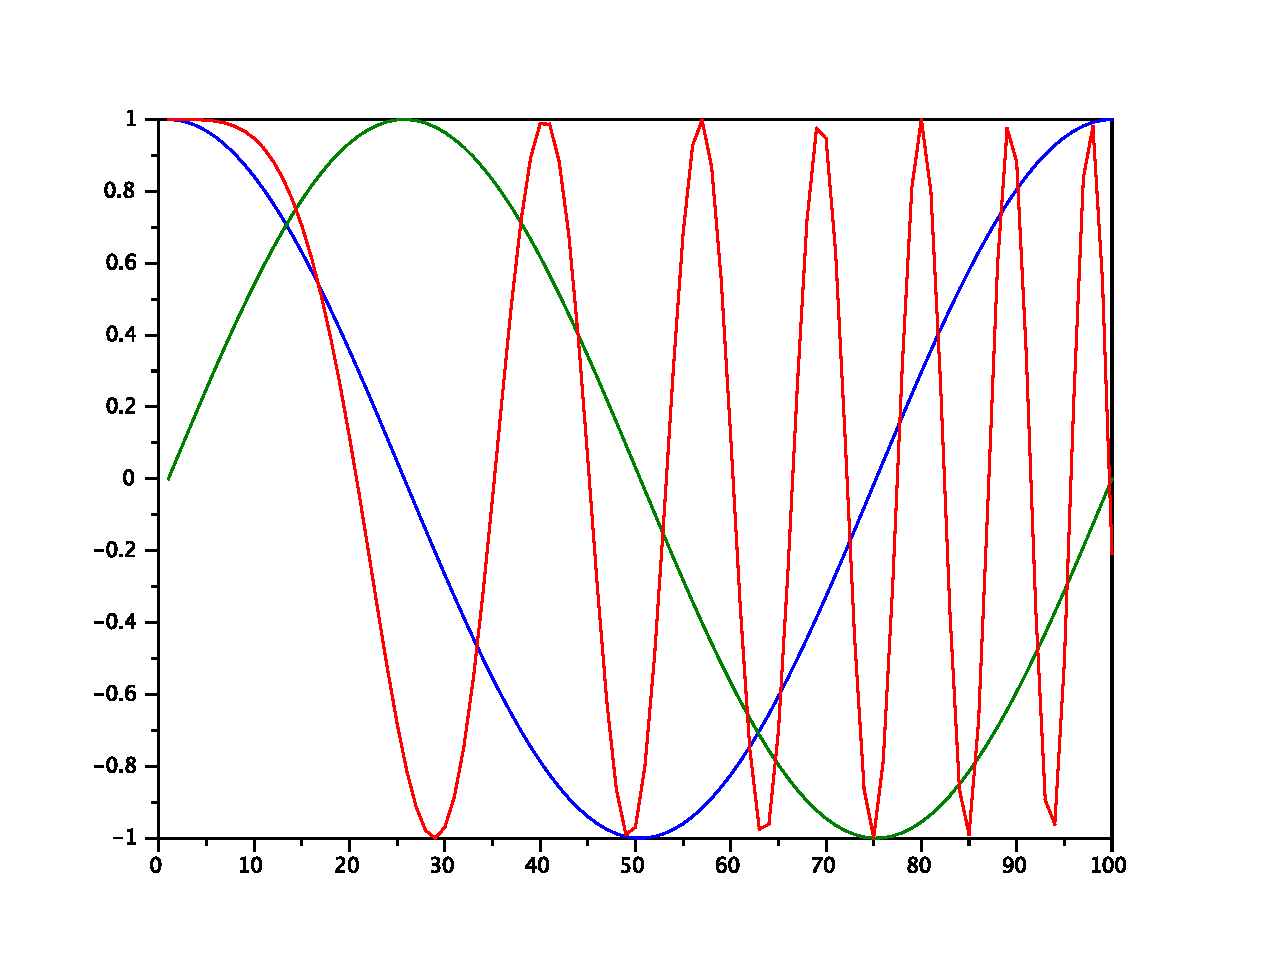
\includegraphics[width=0.33\textwidth]{images/plotmat.pdf}
\item{\textbf{plot}(\textit{v\_x},\textit{v\_y})}  trace la courbe reliant les points $\{(x(t),y(t))\}$
\begin{verbatim}
-->t = linspace(0,6*%pi,100);
-->plot(t.*cos(t),t.*sin(t))
\end{verbatim}
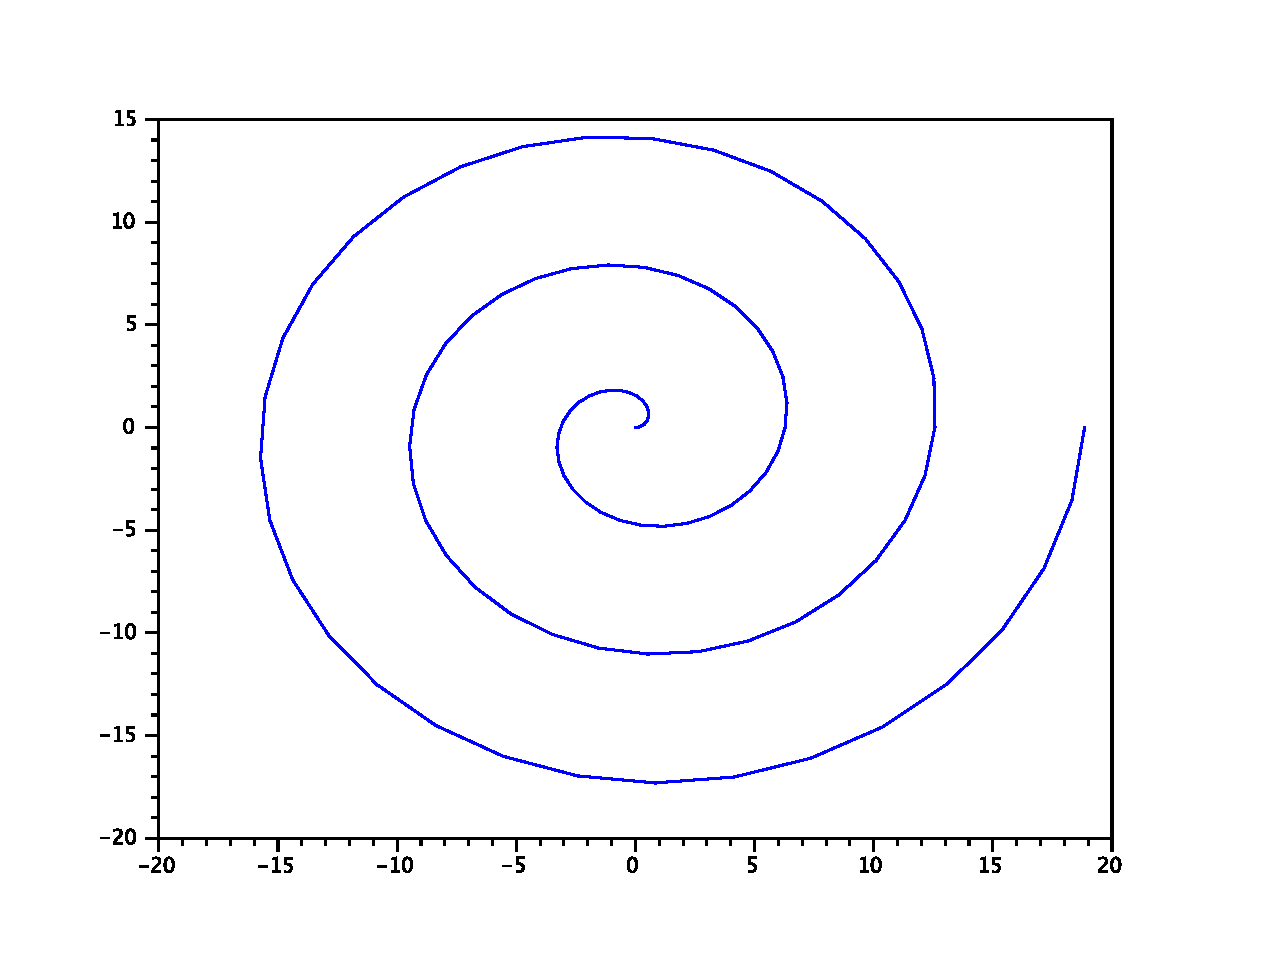
\includegraphics[width=0.33\textwidth]{images/snail.pdf}
\item{\textbf{plot}(\textit{M\_x},\textit{M\_y})}  applique la fonction de tracé précédente successivement à chacune des colonnes des deux matrices.
\begin{verbatim}
-->t = linspace(0,6*%pi,100)';
-->plot([t t+2],[t.*cos(t) t.*sin(t)])
\end{verbatim}
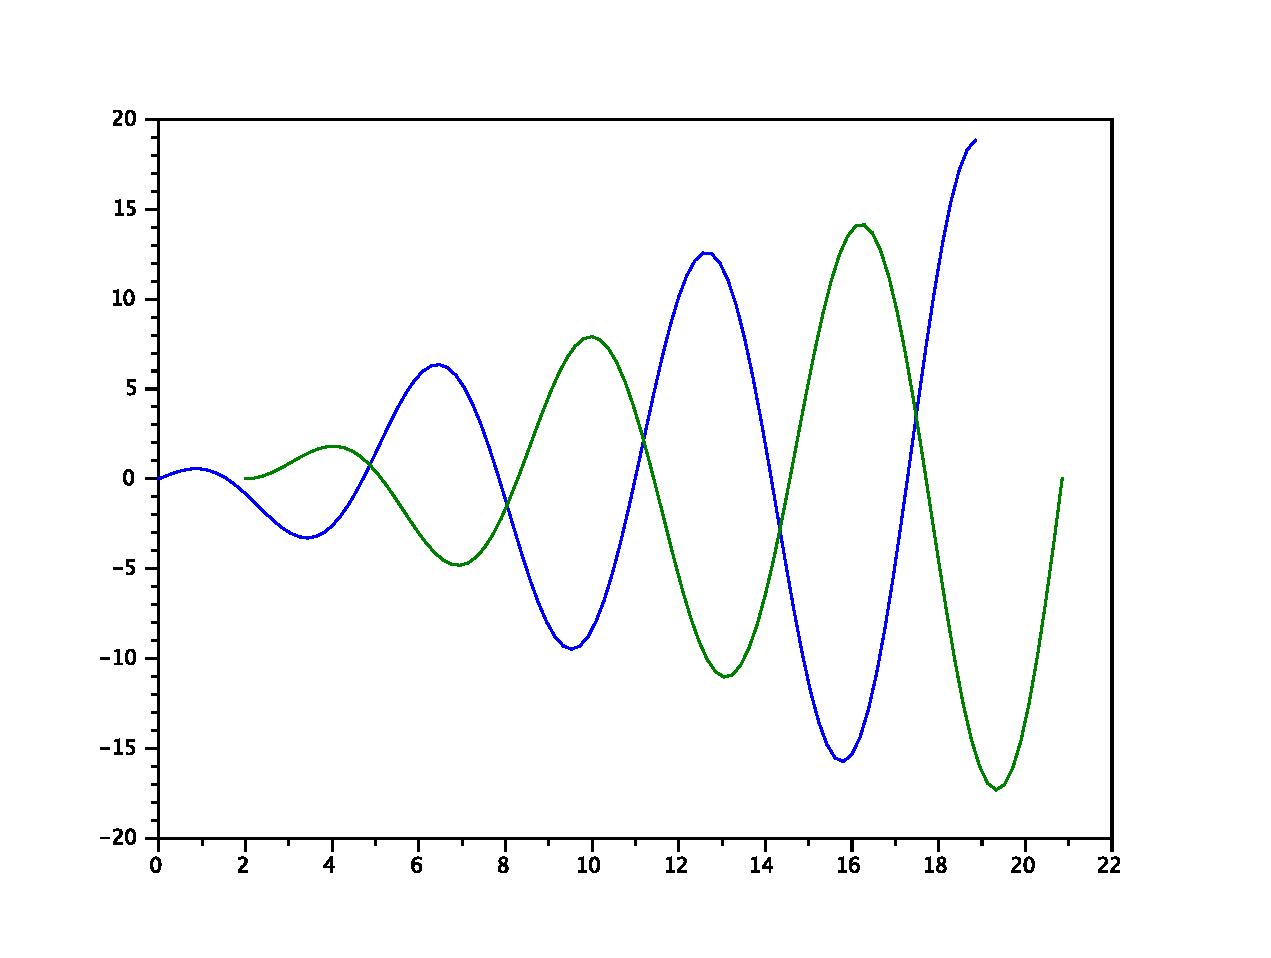
\includegraphics[width=0.33\textwidth]{images/plotmat2.pdf}
\item{\textbf{plot}(\textit{v1\_x},\textit{v1\_x},\textit{str1},\ldots,\textit{vn\_x},\textit{vn\_x},\textit{strn})}  applique la fonction de tracé \textbf{plot}(\textit{v\_x},\textit{v\_y}) avec le style décrit dans la chaîne de caractères (voir
\begin{verbatim}
-->t=linspace(0,6*%pi,200);
-->plot(t,sin(t),'r-',t+%eps,cos(2*t),'b+', ...
-->       t,abs(sin(t)),'ks-')
\end{verbatim}
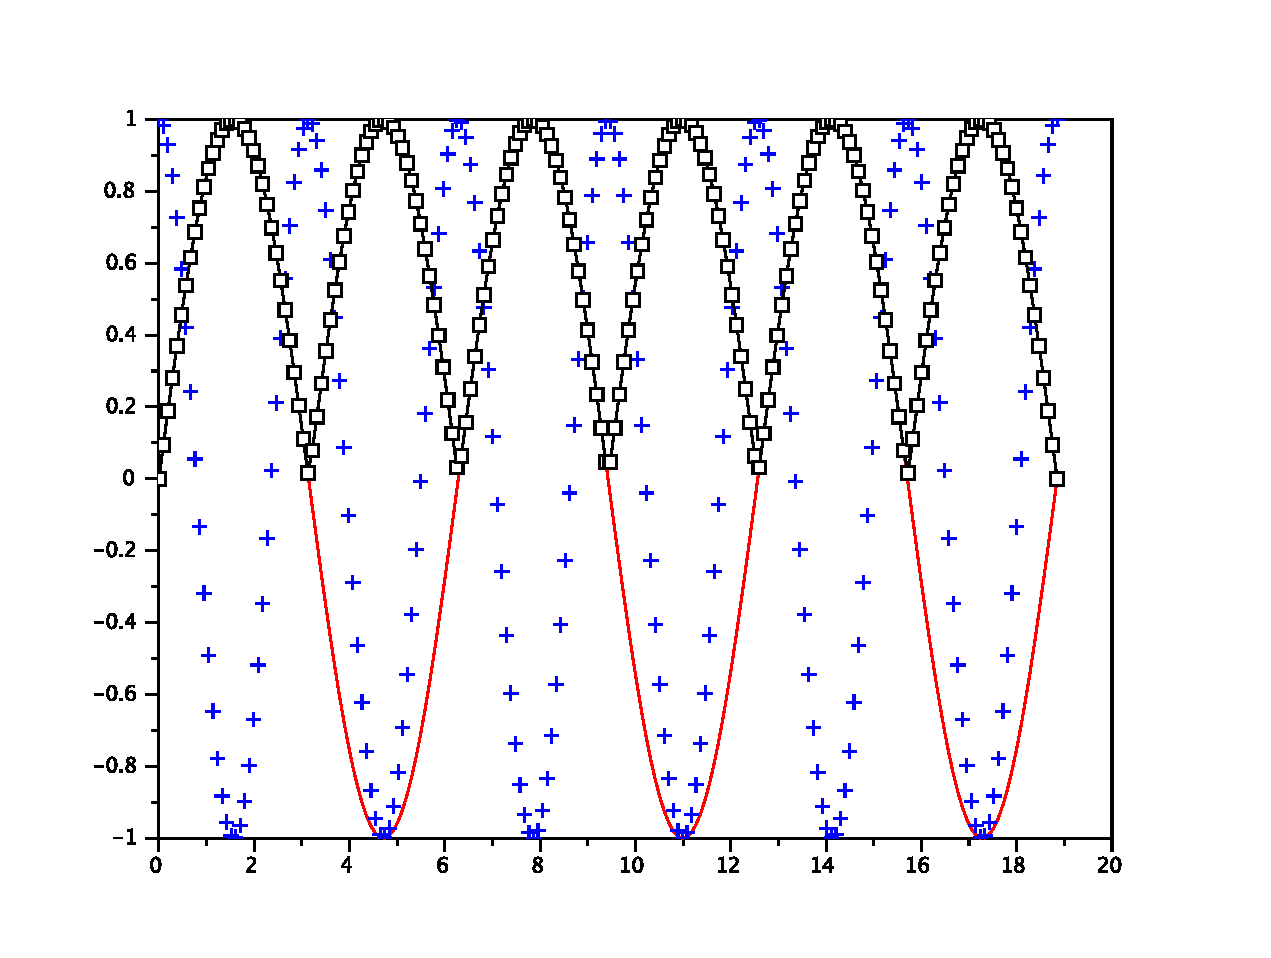
\includegraphics[width=0.33\textwidth]{images/courbes3.pdf}
\item{\textbf{paramfplot2d}($f$,\textit{v\_x},\textit{v\_t})} produit une animation de la courbe paramétrée $x \mapsto f(x;t)$.
\item{\textbf{Matplot}($M$)} affiche une matrice sous la forme d'une image.
\item{\textbf{scf}(\textit{c\_num})} positionne le prochain tracé sur la figure $num$.
\item{\textbf{gcf}()} retourne le numéro de la figure active.
\item{\textbf{clf}()} efface la figure courante.
\item{\textbf{clf}(\textit{c\_num})} efface la figure $num$.
\item{\textbf{drawlater}()} retarde l'affichage d'un graphique tout en permettant de le préparer en mémoire.
\item{\textbf{drawnow}()} affiche le graphique préparé en mémoire.
\item{\textbf{xarrows}(\ldots),\textbf{xrect}(\ldots)} sont des primitives de tracé d'objets graphiques.
\item{\textbf{plot3d}(\ldots)} est la fonction générique de tracé 3d.
\item{\textbf{genfact3d}} permet de générer les facettes d'une surface pour un dessin en 3d.
\item{\textbf{surf}(\textit{M\_Z})} dessine une surface en 3d à partir des valeurs de la maurice $Z$
\item{\textbf{surf}(\textit{M\_X},\textit{M\_Y},\textit{M\_Z})} idem en spécifiant en $X$ et $Y$ les coordonnées de la grille sur laquelle on connaît $Z$.
\begin{verbatim}
t=linspace(0,6*%pi,100)';
plot3d(t.*cos(t),t.*sin(t),t)
t=[0:0.3:2*%pi]'; 
z=sin(t)*cos(t');
[xx,yy,zz]=genfac3d(t,t,z);
plot3d(xx,yy,zz)
\end{verbatim}

\end{description}


\section{Programmation}
\subsection{Fonctions et paramètres}
\label{fonctions}
%deff('[s1,s2,...]=newfunction(e1,e2,....)',text [,opt])
\begin{description}
\item{\textbf{function} [\textit{var\_o1},\ldots,\textit{var\_om}]=\textit{nom\_fonct}(\textit{var\_i1},\ldots,\textit{var\_in})}
	 \textit{cmd\_1}\\ \ldots\\\textit{cmd\_n};\\
\hspace*{-7mm}\textbf{endfunction}\\
où $i1$,\ldots,$in$  et $o1$,\ldots,$om$ désignent respectivement les paramètres d'entrée et les sorties de la fonction \textit{nom\_fonc}. \emph{Convention} : le code de la fonction \textit{nom\_fonc} se trouve dans le fichier \textit{nom\_fonc.sci}.\\

\emph{Extrait du fichier ''mafonction.sci''}
\begin{verbatim}
function [x2] =mafonction(x)
   x2 = x**2;
endfunction
\end{verbatim}
\vspace{3mm}
\emph{Puis dans la console}
\begin{verbatim}
-->mafonction(3)
 ans  =
    9.
\end{verbatim}

\item{\label{deff}\textbf{deff}(\textit{str\_specif}, \textit{str\_code})} permet de définir une fonction (courte) en ligne sans passer par un fichier .sci. La chaine de caractères \textit{str\_specif} contient la spécification de la fonction, la chaine de caractères \textit{str\_code} en contient le code.
\begin{verbatim}
-->deff('[x2]=mafonction(x)','x2 = acos(x)');
-->mafonction(3)
 ans  =
    9.
\end{verbatim}
\item{\textbf{deff}(\textit{str\_specif}, \textit{str\_code},'p')} rajoute l'option de profilage à la fonction définie en ligne.
\end{description}

\subsection{Structures de contrôle}
\label{controle}
\begin{description}
\item{Branchement conditionnel \textbf{if}}\\

\vspace{-3mm}
\hspace*{-7mm}\textbf{if} \textit{cond} \textbf{then}\\
\textit{cmd\_1}; \ldots; \textit{cmd\_n};\\
\hspace*{-7mm}\textbf{elseif} \textit{cond\_i} \textbf{then}\\
\textit{cmd\_i1}; \ldots; \textit{cmd\_in};\\
\hspace*{-7mm}\textbf{else}\\
\textit{cmd\_e1}; \ldots; \textit{cmd\_en};\\
\hspace*{-7mm}\textbf{end}\\

\item{Répétitive \textbf{for}}\\

\vspace{-3mm}
\hspace*{-7mm}\textbf{for} \textit{var}=$v$ \textbf{do}\\
\textit{cmd\_1}; \ldots; \textit{cmd\_n};\\
\hspace*{-7mm}\textbf{end}\\

\vspace{-3mm}
\hspace*{-7mm}\textbf{for} \textit{var}=$M$ \textbf{do}\\
\textit{cmd\_1}; \ldots; \textit{cmd\_n};\\
\hspace*{-7mm}\textbf{end}\\

\item{Répétitive \textbf{while}}\\

\vspace{-3mm}
\hspace*{-7mm}\textbf{while} \textit{cond} \textbf{do}\\
\textit{cmd\_1}; \ldots; \textit{cmd\_n};\\
\hspace*{-7mm}\textbf{end}
\end{description}
\label{excontrole}
\begin{verbatim}
v = 1;
if v==0,
   for i=1:3,
      disp(i);
   end
else
  i=3;
  while i>=1,
     disp(i);
     i = i-1;
  end, 
end    
\end{verbatim}
\subsection{Autres structures de données}
\begin{description}
\item {\textbf{struct}(\textit{str\_chp1}, $var1$, \ldots,\textit{str\_chpn}, $varn$)} retourne un enregistrement composé d'un ensemble de couples champ / valeur.\\
\begin{verbatim}
-->M  = rand(26,2);M = M.' * M;
-->S = struct('Mat',M,'Det',det(M))
 S  =
   Mat: [2x2 constant]
   Det: 21.51
-->S.Mat
 ans  =
    7.54     7.885  
    7.885    11.1
-->S.det= 6;
\end{verbatim}
\item{\textbf{list}($var1$, $var2$, \ldots, $varn$)} est une liste composée des éléments passé en paramètres.
\begin{verbatim}
-->L  = list(1:5,rand(2,2),[%f %f %t])
 L  =
       L(1)
    1.    2.    3.    4.    5.  
       L(2)
    0.560    0.728  
    0.125    0.268  
       L(3)
  F F T  
-->for l=L,
-->disp(sum(l))
-->end
    15.  
    1.68  
    1.  
-->L(4) = 'chaine';
\end{verbatim}
\end{description}
\subsection{Flot d'exécution, Débogage}
\begin{description}
\item{\textbf{break}} interrompt la répétitive courante.
\item{[\textit{var\_o1},\ldots,\textit{var\_om}] = \textbf{return}(\textit{var1},\ldots,\textit{varm})} provoque la sortie inconditionnelle de la fonction en cours d'interprétation.
\item{\textbf{pause}} interrompt l'éxécution en l'attente de l'appui sur le clavier.
\item{\textbf{xpause}(\textit{c\_tps})} interrompt l'éxécution pendant \textit{tps} millisecondes.
\item{\textbf{setbpt}(\textit{str\_func}), \textbf{setbpt}(\textit{str\_func},\textit{c\_lig})} ajoute un point d'arrêt à l'entrée de la fonction \textit{nunc} ou à un certain numéro \textit{lig} de ligne.
\item{\textbf{delbpt}(), \textbf{delbpt}(\textit{str\_func}), \textbf{setbpt}(\textit{str\_func},\textit{c\_lig})} supprime toute ou partie des points d'arrêt existants.
\item{\textbf{dispbpt}()} liste les points d'arrêt existants.
\item{\textbf{abort}} interrompt l'interprétation courante.
\item{\textbf{quit}} provoque la sortie de Scilab.
\item{\textbf{tic}()} démarre le chronomètre.
\item{\textbf{toc}()} retourne le temps écoulé depuis le dernier \textbf{tic}.
\item{\textbf{showprofile}(\textit{var\_fun})} décore un code des informations de  profilage après exécution de la fonction \textit{fun}.
\item{\textbf{plotprofile}(\textit{var\_fun})} affiche un graphique de profilage après exécution de la fonction \textit{fun}.
\begin{verbatim}
deff('benchchol(n)', ['for i=1:n'
                      '     M = rand(i,i)'
                      '     chol(M.''*M)'
                      'end'],'p')
-->benchchol(500);
-->showprofile(benchchol)
function []=fun(n) |1  |0   |0|
  for i = 1:n,     |500|0   |0|
    M = rand(i, i) |500|0.96|4|
    chol((M.') * M)|500|9.24|6|
  end,             |1  |0   |0|
endfunction        |1  |0   |0|
\end{verbatim}
\end{description}

\section{}

\end{multicols}
\end{document}  